\documentclass{article}

% Packages
\usepackage{titling}
\usepackage[utf8]{inputenc}
\usepackage[english]{babel}
\usepackage{amsmath,amssymb}
\usepackage{graphicx}
\usepackage{float}
\usepackage{subcaption}
\usepackage[hidelinks]{hyperref}
\usepackage{listings}
\usepackage[a4paper, top = 2cm, bottom = 2cm, left = 2cm, right = 2cm]{geometry}
\usepackage{multicol}
\usepackage{booktabs}
\usepackage{array}
\usepackage[table]{xcolor}
\usepackage{geometry}% Package for margin adjusting
\usepackage{titlesec} % Package to change title format


\geometry{
  left=1.9cm, % adjust the left margin
  right=1.9cm, % adjust the right margin
  top=1.9cm, % adjust the top margin
  bottom=1.9cm, % adjust the bottom margin
}

\titlespacing*{\subsection}{0pt}{10pt}{7pt}
\titlespacing*{\section}{0pt}{10pt}{4pt}



\graphicspath{{Figures/}}
\newcolumntype{M}[1]{>{\centering\arraybackslash}m{#1}}



% Title page information
\pretitle{
  \begin{center}
  \LARGE
  
\includegraphics[width=15.1cm,height=3.05cm]{Logo_unipv.png}\vspace*{1cm}\\[\bigskipamount]}


\title{\Large Machine Learning Course\vspace{0.8cm}\\
    \rule{\textwidth}{0.3pt}\vspace{0.3cm}\\
    \textbf{Cake Classification: a CNN + MLP approach}\vspace{0.1cm}\\
    \rule{\textwidth}{0.3pt}\vspace{0.8cm}}

\posttitle{\end{center}}
    
\author{Andrea Alberti\vspace{0.5cm}\\
    \small Department of Computer Engineering - Data Science\\[0.2cm]
    \small University of Pavia, Italy \\
    \small Email: andrea.alberti01@universitadipavia.it}\vspace{0.5cm}
        
\date{\today}

\begin{document}

\begin{titlepage}
   
        \maketitle
        \thispagestyle{empty}

    \begin{multicols*}{2}
            
        \hrule
        \begin{abstract}
        \noindent
        This project aimed to develop accurate classification models for 15 different cake images using two approaches: Multi Layer Perceptron (MLP) and a pre-trained Convolutional Neural Network 
        (CNN) based on PVMLNet, a simplified version of AlexNet. The models were evaluated using various feature types, including low-level features such as color histogram and 
        co-occurrence matrix, as well as combinations of these features. Additionally, neural features extracted from different layers of PVMLNet were explored. 
        The results demonstrate that the best accuracy of 90\% was achieved by utilizing neural features, showcasing the power of leveraging pre-trained CNNs for image classification tasks. 
        In contrast, the utilization of low-level features yielded a comparatively lower accuracy of 31\%. These findings highlight the importance of utilizing deeper representations learned 
        by neural networks, which can capture complex patterns and nuances in the cake images. 
        \\
        \\
        \end{abstract}
     \newcolumn
        \hrule\vspace{0.1cm}
        \tableofcontents
    \end{multicols*}

\end{titlepage}

\newpage
\pagenumbering{arabic}



%---------------------------------------------------------

\begin{multicols}{2}
    
\section{Introduction}
This project focuses on implementing a Neural Network for classifying images of cakes. To tackle this problem, two neural networks are utilized: a Convolutional Neural Network (CNN) 
and a Multi Layer Perceptron (MLP). Additionally, the project compares and evaluates different types of features employed by each network. The primary library employed for 
the implementation is "pvml."

\subsection{Available Data}
The dataset consists of 15 categories of cakes, with each category containing 120 images. Within each category, 100 images are allocated for the training set,
while the remaining 20 images form the test set. All the images in the dataset have been resized to a uniform size of 224 x 224 pixels.

\subsection{Goal}
The objective of this project is to identify the most effective method for extracting features from the cake images. The selected feature extraction technique will then be utilized 
to train a Neural Network capable of accurately classifying new, unseen data into the 15 different cake classes.

\subsection{CNN and MLP}
A Multi-Layer Perceptron (MLP) is a type of Feed-Forward Neural Network. It comprises an input layer, an output layer, and zero or more hidden layers consisting of 
interconnected neurons. In an MLP, each neuron in a layer receives input signals from all neurons in the previous layer. It then applies an activation function to the 
weighted sum of its inputs and passes the result to the next layer.
During training, the parameters of the MLP, which include weights and biases, are learned by optimizing a chosen Loss Function, typically Cross Entropy. 
This optimization process is performed using Backpropagation, where the derivatives are propagated backward through the network, adjusting the parameters iteratively.
On the other hand, a Convolutional Neural Network (CNN) is specifically designed for processing and analyzing visual data, such as images. CNNs consist of multiple layers, 
including convolutional layers, pooling layers, and fully connected layers. The convolutional layers apply filters to the input data, capturing spatial patterns and features. 
The pooling layers downsample the feature maps, reducing their dimensionality. Finally, the fully connected layers combine the extracted features to make predictions. The 
activations of different layers can be used as input features for a classification network such as an MLP.


%-----------------------------------------------------------


\section{Features Extraction}
Before proceeding with the model construction, it is fundamental to pre-process the data to make them suitable for the algorithmic processing. This preprocessing step, known as 
"Feature Extraction," is essential in the model creation process.
In this project, two primary categories of feature extraction methods are compared: "Low-Level Features" and "Neural Features." The first category involves extracting specific 
features directly from the images in an 'handcrafted' way. On the other hand, the second category utilizes a pre-trained neural network to extract features from the images.
In this case the used CNN is the \textit{PVMLNet}, designed as a slight simplification over the \textit{AlexNet} architecture. 
These two approaches are compared to determine the most effective feature extraction method for classifying cake images.

\subsection{Low Level Features}
There are many types of low level features and in this project different combinations of the following ones are considered: Color Histogram, 
Edge Direction Histogram, and Co-occurrence Matrix.

\subsubsection{Color Histogram}
A color histogram is a frequency representation of the color distribution in an image and can be used as a quantitative representation of the image. In Figure 1, the test 
and train accuracies of a multilayer perceptron trained on color histogram features are depicted. The model was trained for 5000 epochs, achieving a test accuracy of 
approximately 21\% while exhibiting a slight overfitting tendency. The growth of the test accuracy appears to plateau after 1000 epochs, suggesting that the model 
struggles to extract further information from the data. This limitation can be attributed to the simplicity of color histogram features, which may not adequately 
capture the intricate complexities present in the images.

    \begin{figure}[H]
        \centering
        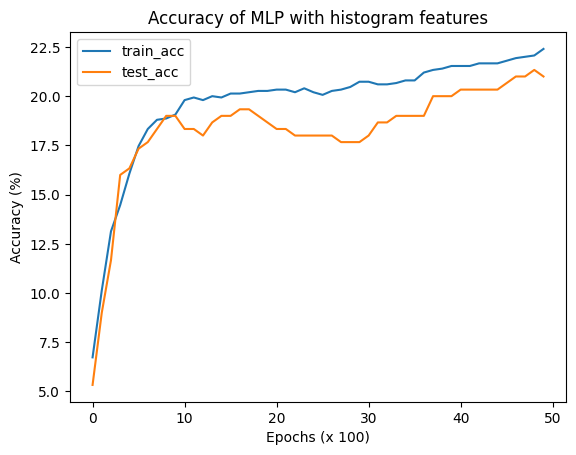
\includegraphics[width=0.48\textwidth]{color_hist.png}
        \caption{Color Histogram}
        \label{fig:color_hist}
    \end{figure}



\subsubsection{Combined Features}
To try enhancing the model performance, the color histogram features were combined with other low-level features, listed in Table \ref{tab:feature_combinations}. 
To merge these features, they were normalized using three different techniques: "Mean-var," "Min-max," and "Max-abs." 

    \begin{table}[H]
        \small
        \centering
        \renewcommand{\arraystretch}{1.5}
        \begin{tabular}{|p{7.8cm}|}
        \rowcolor{blue}
        \hline
        \textcolor{white}{\textbf{Feature Extraction Combinations}} \\
        \hline
        \rowcolor{blue!15}
        Color Histogram + Edge Direction Histogram  \\
        \rowcolor{white}
        Color Histogram + Co-occurrence Matrix \\
        \rowcolor{blue!15}
        Edge Direction Histogram + Co-occurrence Matrix \\
        \rowcolor{white}
        Color Histogram + Edge Direction Histogram + Co-occurrence Matrix  \\
        \hline
        \end{tabular}
        \caption{Feature Extraction Combinations}
        \label{tab:feature_combinations}
    \end{table}
\noindent
The results are presented in Figure \ref{fig:comb_results}, showing the train and test accuracies achieved for each feature type using various normalization techniques and without normalization. 
Notably, the combination of Color Histogram and Edge Direction Histogram yielded similar results to the combination of all three feature extraction techniques, while demonstrating 
a reduced tendency for overfitting. The introduction of normalization techniques improved the test accuracy, with the "Min-max" and "Max-abs" methods outperforming "Mean-var" and achieving 
an approximate accuracy level of 31\%. However, despite the enhanced performance from the feature combination, the results remain unsatisfactory, as the model still struggles to 
accurately classify the images. As a potential attempt for improvement, the next step is to consider neural features.

    \begin{figure}[H]
        \centering
        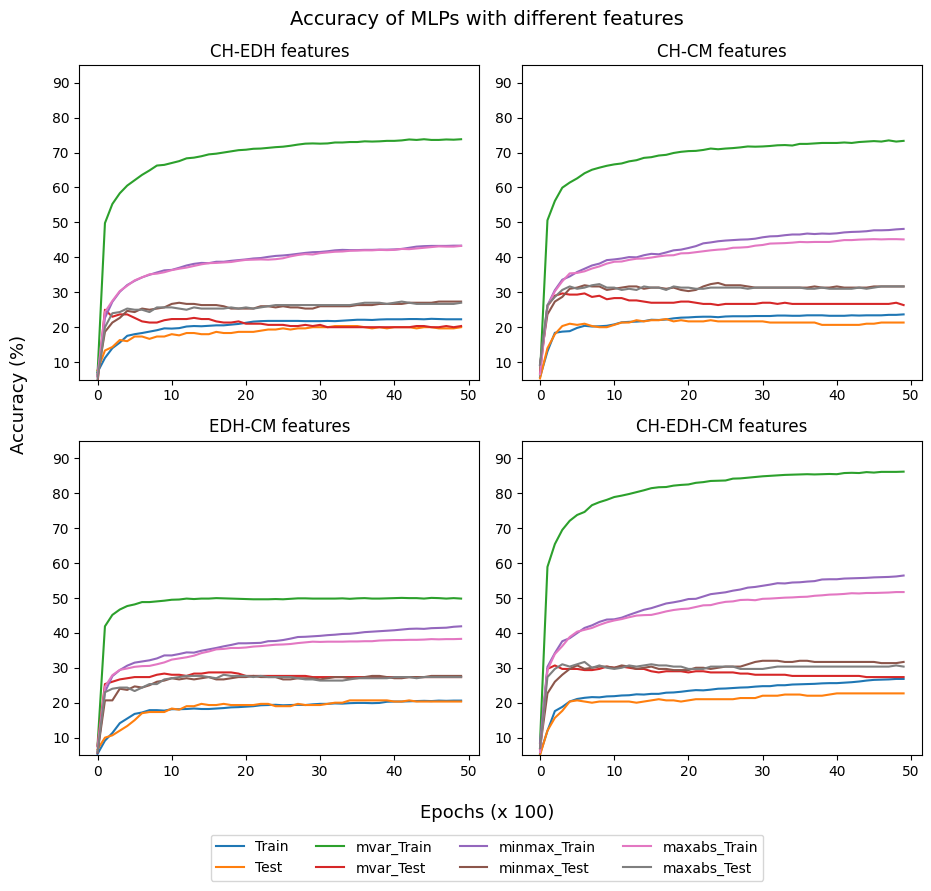
\includegraphics[width=0.48\textwidth]{comb_results.png}
        \caption{Feature Extraction Combinations Results}
        \label{fig:comb_results}
    \end{figure}



\subsection{Neural Features}
In contrast to low-level features, neural features are obtained by utilizing a pre-trained neural network. These features are derived from the activations of different layers within 
the network, which can serve as valuable inputs for the classification task. In this project, the CNN layers considered for feature extraction are denoted as -1, -2, -3, -4, -5, -6, 
and -7, where the numbers represent the layer indices in Python, with -1 representing the last layer.\\
\\
\textbf{Different Activation Layers}\\
In Figure \ref{fig:act_layers} are shown the results of the accuracies achieved by the MLP trained with different activation layers as features. Two ways of extracting the
features have been considered. the first involved making a spatial mean across the values, the second one instead just considered all the values, flattening them. The best
approach in terms of results were this latter and it was chosen for the following analysis. It is worth nothing that this approach requires an higher computational cost since 
the number of features is much higher.
The layers -5 and -6 were observed to be
the most effective, achieving a test accuracy of approximately 90\%. This value is significantly larger than the one obtained using low-level features, proving the 
effectiveness of the neural features. Another proof of their bounty is the extremely reduced number of epochs it was necessary to reach a plateau in the accuracy growth.

    \begin{figure}[H]
        \centering
        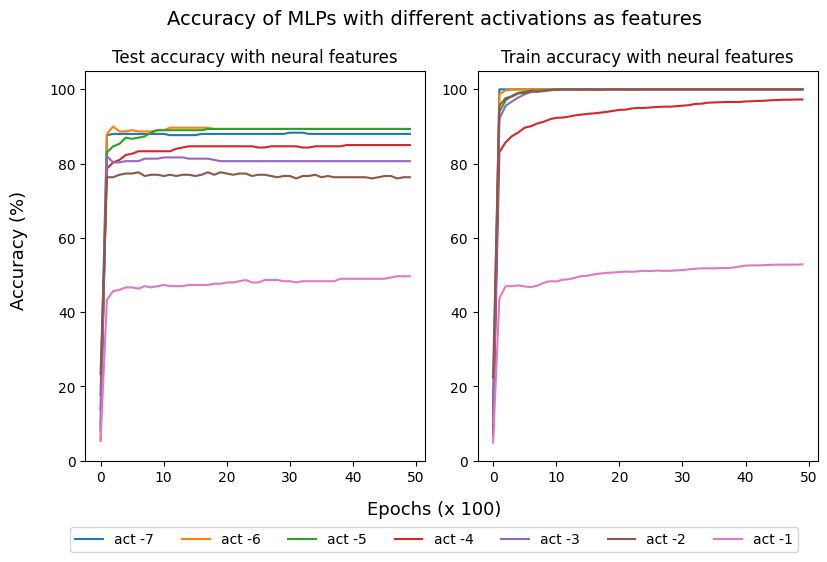
\includegraphics[width=0.48\textwidth]{act_layers.png}
        \caption{Different Activation Layers}
        \label{fig:act_layers}
    \end{figure}


\section{Transfer Learning}
In the context of this project, transfer learning is applied by replacing the last layer of PVMLNet, with the weights of a trained MLP. By doing so, the PVMLNet can benefit from 
the learned weights of the perceptron, potentially improving its performance and enabling it to classify cake images more accurately. 
This transfer of knowledge allows for efficient utilization of the previously learned features and can expedite the training process for this specific classification task.
The reached test accuracy is around 80\%, largely smaller than the 90\% achieved before.



%-----------------------------------------------------------

\section{Model Analysis}
To analyze the behavior of the chosen model ('-5' layer neural features) was used the confusion matrix in figure \ref{fig:confmat} showing the number of correct and 
incorrect predictions for each class. The darker the color, the higher the number of samples of class i (row index) classified as class j (column index). 
As expected, the diagonal is the most populated part of the matrix, meaning that the model correctly classifies the images most of times.

\subsection{Most Exchanged Classes}
The most exchanged classes are those in which the model has more difficulties to distinguish between. In figure \ref{fig:mostex} are reported for each cake the class to which
the model classifies it (excluded correct classifications) most of times. An investigation on the most exchanged classes could be useful to understand the reason behind the
misclassifications and to improve the model performance. The factors affecting the choice are a lots, including the shape of the cake, the colors and 
even the texture.

    \begin{figure}[H]
        \centering
        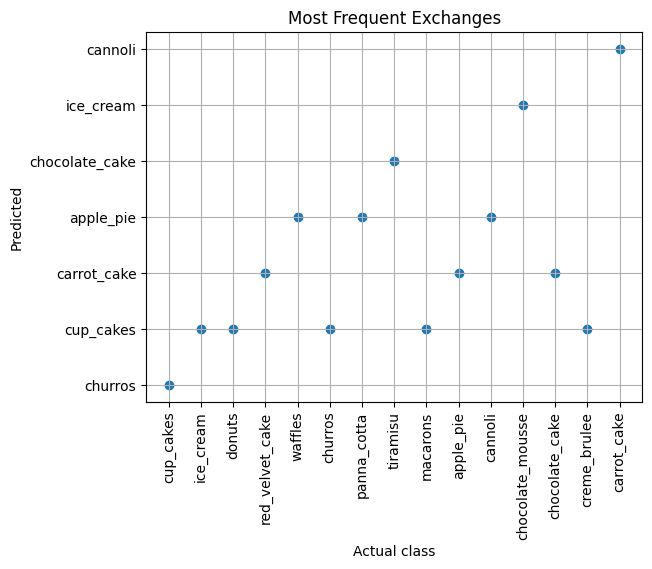
\includegraphics[width=0.48\textwidth]{mostex.png}
        \caption{\small Most exchanged}
        \label{fig:mostex}
    \end{figure}


\subsection{Most Misclassified Samples}
Some cakes are more difficult to be classified than others and in figure \ref{fig:mostmis} are reported the most misclassified samples. \textit{Chocolate-mousse}, \textit{Apple-pie} and \textit{Tiramisu} are the most 
misclassified cakes, and they are exchanged respectively with \textit{Ice-cream}, \textit{Carrot-cake} and \textit{Chocolate-cake}. To understand the reason behind these misclassifications, further investigations are needed.

    \begin{figure}[H]
        \centering
        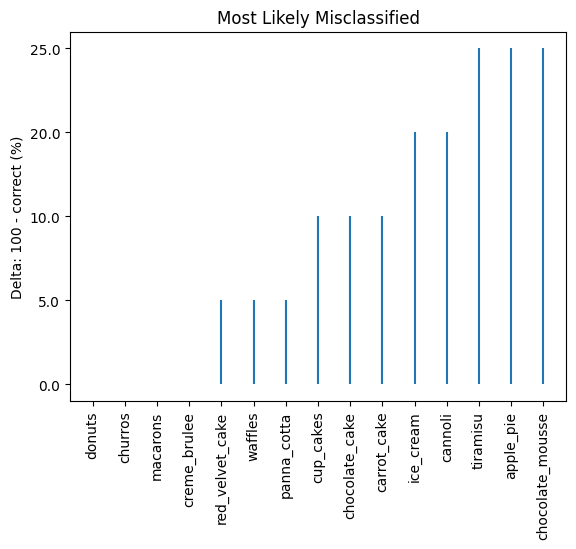
\includegraphics[width=0.48\textwidth]{mostmis.png}
        \caption{\small Most misclassified}
        \label{fig:mostmis}
    \end{figure}


\subsection{Misclassified Images}
A last interesting and useful analysis is to look at the images that the model misclassifies and to their predicted classes. In figure \ref{fig:wrong_pred} are reported 4 images misclassified
by the model. The title indicate the actual class, while the bars indicate the probability of the 5 most likely classes predicted by the model. Understanding the reason behind these
misclassifications could be not so easy, but achieving this goal could be useful to improve the model performance. To provide an enhanced vision on the misclassified cakes, 
in Figure \ref{fig:wrong_pred_images} are reported their actual images.

    \begin{figure}[H]
        \centering
        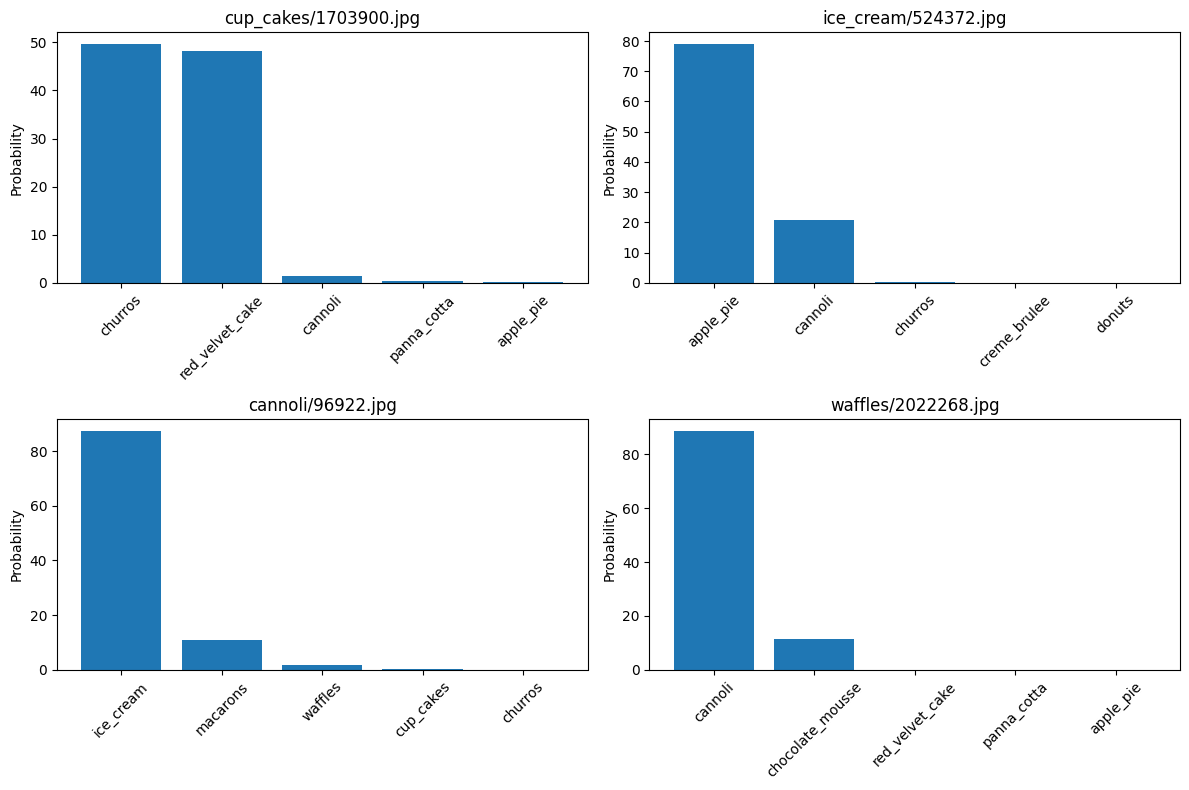
\includegraphics[width=0.48\textwidth]{wrong_pred.png}
        \caption{\small Predictions for the images}
        \label{fig:wrong_pred}
    \end{figure}

    \begin{figure}[H]
        \centering
        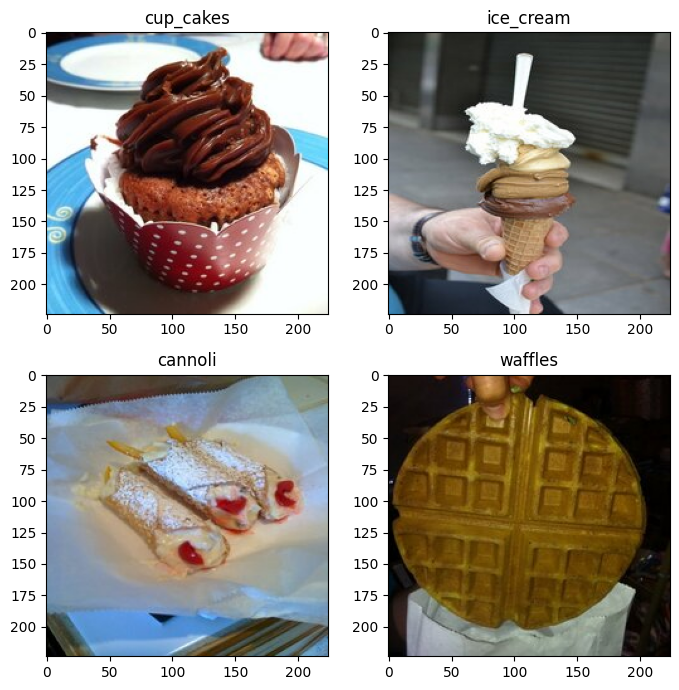
\includegraphics[width=0.48\textwidth]{wrong_pred_images.png}
        \caption{\small Actual images}
        \label{fig:wrong_pred_images}
    \end{figure}



\end{multicols}

        \begin{figure}[H]
            \centering
            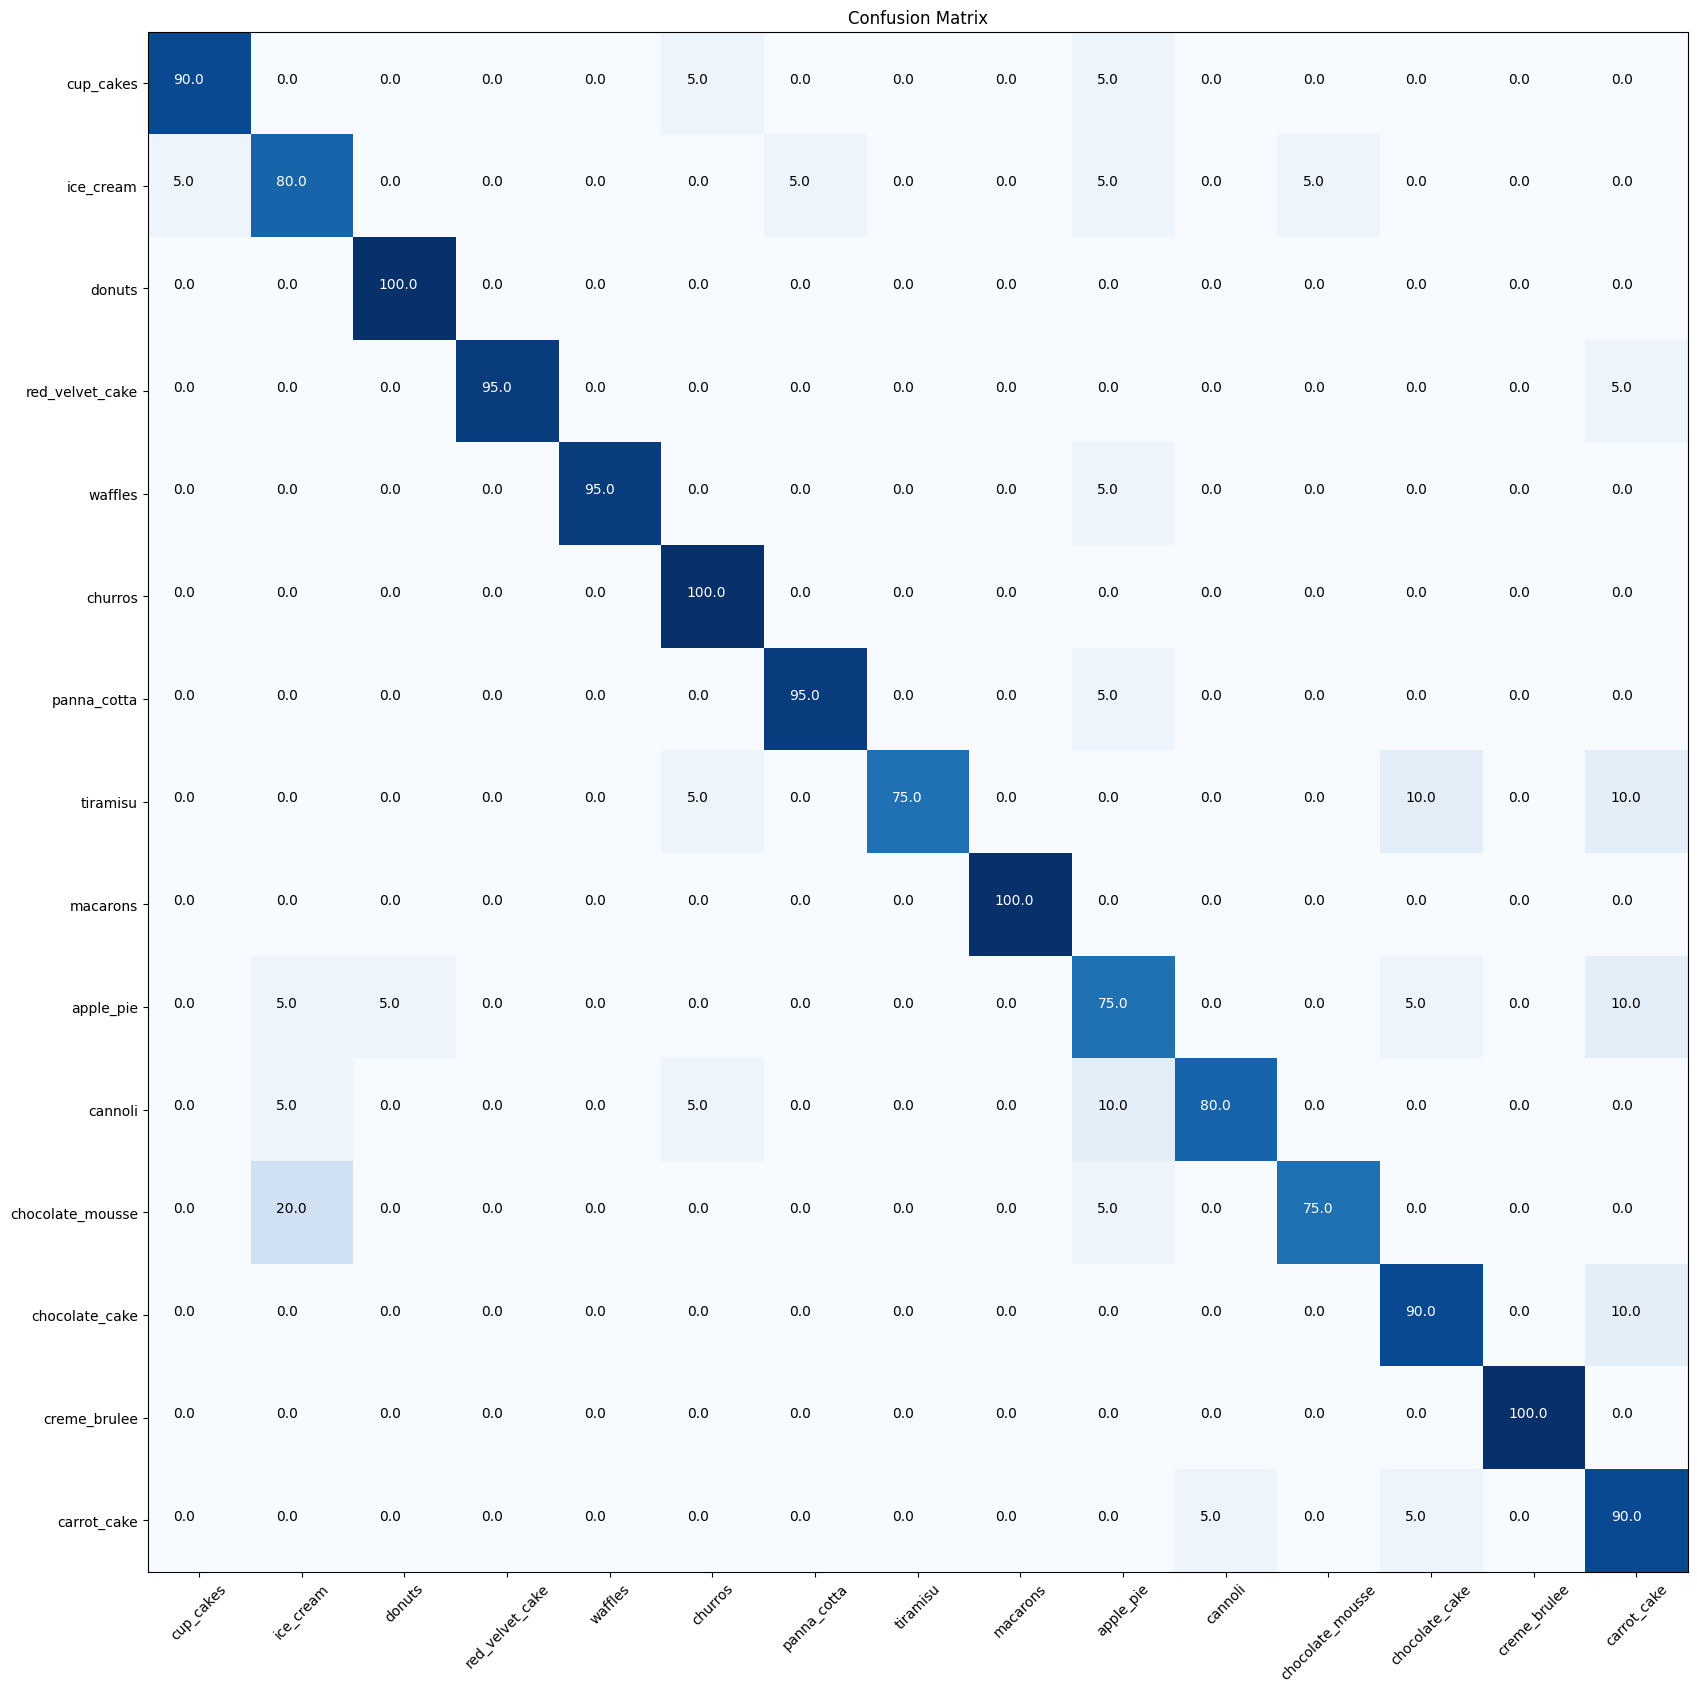
\includegraphics[width=0.9\textwidth]{confmat.png}
            \caption{\small Test accuracies comparison}
            \label{fig:confmat}
        \end{figure}


%-----------------------------------------------------------


\vfill
%\subsection*{\normalsize Declaration}
%I affirm that this report is the result of my own work and that I did not share any part of it with anyone else except the teacher.


\end{document}